\documentclass[a4paper]{article}
\usepackage{multicol}
\usepackage{makeidx}
\usepackage{lstautogobble}
\usepackage{textgreek}
\usepackage[margin=1.25in]{geometry}
\usepackage[greek, english]{babel}
\usepackage{amsmath}
\usepackage{graphicx}
\usepackage[colorinlistoftodos]{todonotes}
\usepackage{listings}
\lstset{basicstyle=\ttfamily,
  escapeinside=||,
  autogobble}
\newcommand{\tab}[1]{\hspace{.2\textwidth}\rlap{#1}}

\title{\huge{Graphene}	\\	\LARGE{Language Reference Manual} \\ \large{COMS W4115 Programming Languages and Translators}} 

\author{Adith Tekur (at2904)\\ Pooja Prakash(pk2451)\\ Sarah Panda (sp3206)\\ Sumiran Shah (srs2222)\\ Neha Rastogi (nr2477)\\ \\
Team 8}

\date{\today}
\makeindex


\begin{document}
\thispagestyle{empty}
\begin{large}
\begin{figure}
\centering
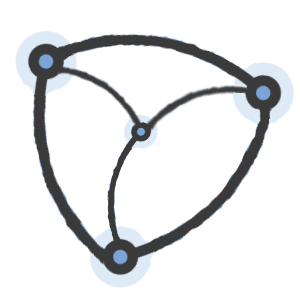
\includegraphics[width=0.3\textwidth]{graph-logo.png}
\end{figure}
\pagenumbering{roman}
\newpage
\maketitle
\newpage
\tableofcontents
\maketitle

\pagebreak
\clearpage
\pagenumbering{arabic}
\setcounter{page}{1}
\section{Introduction}

	In this manual, we describe the various features of Graphene that can be used in defining and manipulating graphs. We present an overview of the lexical conventions, syntax of the language and the grammar representing Graphene.

\section{Lexical Conventions}

Like for every language, Graphene is composed of lexemes following patterns represented by tokens. Apart from whitespaces (that represent spaces, tabs and newlines) and comments, our language has the tokens - identifiers, keywords, constants, operators and separators.


\subsection{Comments}

Graphene provides support for both single and multi-line comments. Single-line comments begin with "//". Multi-line comments on the other hand bengin with "/*" and and with "*/". An example is as follows.

\begin{quote}
\begin{verbatim}

// This is a single-line comment 

/* This is a...
… multi-line comment */ 

\end{verbatim}
\end{quote}
Note that one multi-line comment cannot be nested within another multi-line comment.

\subsection{Identifiers}

\noindent An identifier represents a unique entity within a program. Graphene follows the naming convention specified below.

\begin{enumerate}
\item An identifier must begin with a '\$'
\item Following the '\$', an identifier can be any sequence of alphabets, digits or underscores.
\end{enumerate}

\noindent Graphene is case-sensitive.

\subsection{Keywords}
The following keywords convey special meaning to Graphene and hence should not be used elsewhere.

\begin{multicols}{2}
\begin{quote}
\begin{verbatim}
if
else
for
while
Graph
Node
Edge
has
connects
lambda
def
True
False
\end{verbatim}
\end{quote}
\end{multicols}

\subsection{Reserved}
The following characters are reserved for use in the grammar.

\begin{multicols}{5}
\begin{quote}
\begin{verbatim}
+ 	
- 	
*
/	
%
( 	
) 	
{ 	
} 	
[	
]
=
==	
!=	
<	
>	
>=	
<=
&&	
||	
!
.	
,	
;	
$
->
<->
'
"
\end{verbatim}
\end{quote}
\end{multicols}

\section{Types}

\subsection{Basic Types}
Graphene handles type dynamically. 
Basic data-types recognized and handled approriately are:

\begin{quote}
\begin{enumerate}
\item int - This is used to define integer numbers. Data of the form $[0-9]*$ will be handled as type $int$.
\item float - This is used to define floating-point numbers. $[0-9]+.[0-9]+$ translates to type $float$.
\item boolean - Values 'True' or 'False' will define $boolean$ type.
\item string - This is used to represent strings (sequence of characters enclosed within $""$ or $'$ $'$).
There is no char type. Instead, it is handled as a string made of 1 character. This eliminates the need to handle $'$ and $"$ differently.
\end{enumerate}
\end{quote}
All the basic data-types - int, float, char and boolean can also be represented in Graphene as a string (sequence of characters enclosed within ""). 
\newline
\newline
The type of the variable is determined dynamically on the basis of the the characters enclosed and is handled accordingly. 

The following is one such example.

\begin{multicols}{2}
\begin{quote}
\begin{verbatim}
integerVar = 70;		
floatVar = 50.5;		
boolVar = True;		
stringVar = "graphene";
//integerVar is handled as an integer
//floatVar is handled as a floating point
//boolVar is handled as boolean.
//stringVar is handled as a string
\end{verbatim}
\end{quote}
\end{multicols}

\subsection{Derived Types}
The following are the derived data-types supported by Graphene.
\begin{quote}
\begin{enumerate}
\item Graph - This is used used to define graphs.
\item Node - This is used to define a node in terms of user-defined properties representing the node. Graphene assigns a unique id to every node that is created. In other words, the id$s$ of the nodes are globally unique.
\item Edge - This is used to define an edge in terms of user-defined properties representing the edge. Like in nodes, Graphene ensures that all edges have globally unique identifiers. 
\item Arrays - Graphene supports arrays to represent multiple entities of the same type. An element within an array can be accessed using its index (Ex. arr[0] retrieves the first element of the array arr).
\end{enumerate}
\end{quote}

\subsection{Escape Sequences}
The following escape sequences are supported by Graphene.

\begin{multicols}{2}
\begin{quote}
\begin{verbatim}
\n	
\t	
\\	
\'	
\"	
newline
tab
backslash
single quote
double quote
\end{verbatim}
\end{quote}
\end{multicols}

\subsection{Boolean Constants}
The boolean constants supported by Graphene are True and False.

\section{Scope}
\subsection{Block Scope}
Variables declared in a block are valid only for that block. A block can be a part of the function definition.

\subsection{Function Scope}
Variables declared in a function are valid only within that function. Once the function returns, the variables declared within the function are no longer visible.

\subsection{Global Scope}
Variables declared outside the functions are valid for all the functions in that program.

\subsection{Lexical Scope}
A variable's scope is based only on its position within the textual corpus of the code. Variable names in the same scope must be unique.

\subsection{Linkage Scope}
External library function or constants can be accessed through their identifiers and are shared by the entire program.

\section{Grammar}
\begin{quote}
\begin{verbatim}
function-dec:
    function
    lambda

lambda:
    'lambda' lambda-arguments compound-statement return-arguments ';'

function:
    'def' function-arguments $ID compound-statement return-arguments ';'

function-arguments:
    lambda-arguments
	
argument-list:
    'lambda' $ID
    'lambda' $ID ',' argument-set

\end{verbatim}
\begin{lstlisting}
lambda-arguments:
    '(' argument-set ')' '=>'

argument-set:	
    type $ID
    type $ID ',' argument-set

return-arguments:
    '=>' '(' return-set ')'
\end{lstlisting} 
    \tab\textepsilon
\begin{lstlisting}
return-set:
    $ID
    $ID ',' return-set

statement-list:
    statement
    statement statement-list

statement:
    expression-statement 
    selection-statement 
    iteration-statement 
    class-method-expression 

compound-statement: 
    '{' '}' 
    '{' statement-list '}' 
 
expression-statement:
    ';'
    expression ';'
 
expression: 
    assignment-expression; 
 
assignment-expression: 
    type $ID '=' type '.new()' 
    type $ID '=' assignment-expression 
    logical-OR-expression 

logical-OR-expression: 
    logical-AND-expression
    logical-OR-expression '||' logical-AND-expression 
 
logical-AND-expression: 
    equality-expression 
    logical-AND-expression '&&' equality-expression 
 
equality-expression: 
    relational-expression
    equality-expression '==' relational-expression 
    equality-expression '!=' relational-expression 
 
relational-expression: 
    additive-expression 
    relational-expression '<' additive-expression 
    relational-expression '>' additive-expression 
    relational-expression '<=' additive-expression 
    relational-expression '>=' additive-expression 
 
additive-expression: 
    multiplicative-expression 
    additive-expression '+' multiplicative-expression 
    additive-expression '-' multiplicative expression 
 
multiplicative-expression: 
    primary-expression 
    multiplicative-expression '*' primary-expression 
    multiplicative-expression '/' primary-expression 

type:
    primitive-type
    array-type

primitive-type:
    'Node'
    'Edge'
    'Graph'

array-type:
    primitive-type '[]'
    $ID '[]'
	
program:
    declaration-list

declaration-list:
    declaration-list declaration
    declaration

declaration:
    var-dec
    function-dec
    statement

statement:
    expression-stmt
    compound-stmt
    selection-stmt
    iteration-stmt
    return-stmt
    break-stmt		

statement-list:
    statement-list statement
    statement

expression-stmt:
    expression ;
    ;	

selection-stmt:
    if ( simple-expression ) statement 
    if ( simple-expression ) statement else statement

iteration-stmt:
    while ( simple-expression ) statement
    foreach ( mutable in simple- expression ) statement

return-stmt:
    return ; 
    return expression ;

break-stmt:
    break ;

compound-stmt:
    { local-declarations statement-list }

function-dec:
    type-specifier $id ( params ) statement 
    $id ( params ) statement 

params:
    param-list 
\end{lstlisting} 
    \tab\textepsilon
\begin{lstlisting}

param-list: 
    param-list ; param-type-list 
    param-type-list

param-type-list:
    type-specifier param-id-list	

param-id-list:
    param-id-list , param-id 
    param-id						 

param-id:
    $ID
    constant 

var-dec: 
    node 
    graph 
    edge 
    list

node:
    $id "has" keylist

edge:
    $id "connects" $id ',' $id "has" key-list

keylist:
    $id
    $id "," keylist

graph:
    "Graph" $id "has" graph-type "{" edge-list "}"

graphtype:
    "u"
    "d"

edge-list:
    $id connector $id
    $id connector $id "," edge-list

connector:
    "->"
    "<->"

list:
    "List" $id 

node:
    "Node" initializer

edge:
    "Edge" initializer

initializer:
    $id $id "=(" kv-list ")"

kv-list:
    kv
    kv "," kv-list

kv:
    $id
    $id ":" $id


multiple-return:
    "(" id-list ")" "=" call

id-list:
    $id 
    $id "," id-list	

expression:
    mutable "=" expression
    mutable "+=" expression
    mutable "-=" expression
    mutable "++"
    mutable "--"
    simple-expression

multiple-return-expr:
    mutable-list "=" call
					 							
simple-expression:
    simple-expression "or" and-expression
    and-expression
				 							
and-expression:
    and-expression "and" unary-rel-expression
    unary-rel-expression
			
unary-rel-expression:
    "not" unary-rel-expression
    rel-expression

rel-expression:
    sum-expression relop sum-expression
    sum-expression
			 							
relop:
    "<="
    "<"
    ">"
    ">="
    "=="
    "!="	
    
sum-expression:
    sum-expression sumop term
    term				 							


sumop:
    "+"
    "-"
			 							
term:
    term mulop unary-expression
    unary-expression

mulop:
    "*"
    "/"
    "%"					 					

unary-expression:
    unaryop unary-expression
    factor					

unaryop:
    "-"
    "*"

factor:
    immutable
    mutable

mutable:
    ID
    ID "[" expression "]"

immutable:
    ( expression )
    call
    constant

call:
    $id "." ucall
    ucall   

ucall:
    $id args
    $id args "." ucall
    
args:
    "(" arg-list ")" \end{lstlisting} \tab \textepsilon
    \pagebreak
\begin{lstlisting}
arg-list:
    expression "," arg-list
    expression

constant:
    NUMCONST
    CHARCONST
    STRINGCONST
    True
    False 

\end{lstlisting}
\end{quote}

\section{Grammar Explanation}
\subsection{Lambda Functions}
\begin{verbatim}
    lambda:
        'lambda' lambda-arguments compound-statement return-arguments ';'
\end{verbatim}

\indent A lambda function, defined by beginning with the keyword "lambda", can be used by a user to specify the logic on the basis of which functions utilizing lambdas can perform manipulations. For example, clustering functions will accept a lambda function as their first argument that specifies the heuristic for grouping of nodes into clusters. The keyword lambda identifies such a function. Like regular functions, lambda functions takes in zero or more comma separated list of arguments. A comma separated list of arguments can be returned.
Built-in functions will specify the signature of the lambda they except. A mismatch will result in a compile error.

\subsection{User-defined Functions}
\begin{verbatim}
    function:
         'def' function-arguments $ID compound-statement return-arguments ';'
\end{verbatim}

\indent User-defined functions, beginning with the keyword "def", are structurally similar to lamba functions except that the first argument may be a lambda function. Note that in the presence of a lambda function, it has to always be the first argument that is passed. Like in lambda functions, Graphene supports multiple return values.

\indent A user-defined function can accept a lambda as an optional first argument. A lambda however, cannot accept another lambda as an argument.

\subsection{Function Calls}
\begin{verbatim}
    call:
        $id "." ucall
        ucall
\end{verbatim}

\indent A function call consists of the name of the function followed by its arguments. The return value of this function can in turn call another function, providing for function chaining.

\subsection{Handling Multiple Return Arguments}
\begin{verbatim}
    multiple-return:
        "(" id-list ")" "=" call
\end{verbatim}

\indent Graphene provides out-of-the-box support for multiple return arguments. A list of variables can then form the LHS for a function call that returns multiple values. In the event of mismatch of number of arguments, an error is generated.

\subsection{Nodes and Edges}
\subsubsection{Declaration}
\begin{verbatim}
    node:
        $id "has" keylist
\end{verbatim}

\indent Graphene allows users to define properties that represent a node. These properties are typically key-value pairs. The user can define a universal set of keys for a particular node type. The "has" keyword implies that the node should contain values for at least the specified set of keys.

\begin{verbatim}
    edge:
        $id "connects" $id ',' $id "has" key-list
\end{verbatim}

\indent The keyword "connects" is used to specify the the two nodes the edge is used to connect. In the above production rule, the first \$id is the id of the edge. The two \$ids following the "connects" keyword are the ids of the nodes. Also, like nodes, edges can also have key-value pairs and are specified similar to the key-value pairs of nodes. 

\subsubsection{Initialization}
\begin{verbatim}
    initializer:
        $id $id "=(" kv-list ")"
\end{verbatim}

The above production rule is used to initialize both nodes and edges by assigning values to the keys of their corresponding types. The first \$id represents the type of the node or the edge as defined in the declaration part. The second \$id is the unique id of the node or the edge. kv-list represents the set of values to be assigned to the keys defined. Also, if a user wants to define additional keys that are not defined, (s)he may do so by using the format "key":"value" where key is the new key and value is its corresponding value. But values $must$ be provided for the declared set of keys.\newline

An example of the declaration and initialization of a node is as follows.

\begin{multicols}{2}
\begin{quote}
\begin{verbatim}
Person has name, school;
Person 2 = ("Jacob", "CU", "age":"20");


//Declaring a node-type Person

//Assigning values to keys of 
//Person for node 2
\end{verbatim}
\end{quote}
\end{multicols}

\subsection{Graphs}
\subsubsection{Declaration \& Initialization}
\begin{verbatim}
    graph:
        "Graph" $id "has" graph-type "{" edge-list "}"
\end{verbatim}

\indent A variable of graph data type can be declared using the edge list and a keyword which represents whether the graph is directed or not. 
graph-type is "u" for undirected graphs and "d" for directed graphs. 
Edge list contains the list of all edges along with the connector which represents the direction of the edges. Connector $"->"$ refers to a directed edge in a single direction and $"<->"$ refers to directed edges in both directions. The latter also represents the edge in an undirected graph.

\end{large}
\end{document}
